\section{Introduction}
\label{sec:introduction}

TODO

\color{red}
For Arash and Hala: please use \\{\tt \textbackslash cref\{sec:introduction\}}\\ to refer to sections, figures etc. It automatically adds things as `Section': e.g., \cref{sec:introduction}.
\color{black}

The introduction contains: 
\begin{itemize}
	\item Setting up the context of automated driving
	\item Giving some background information about the hazard analysis and risk assessment in the ISO~26262 standard
	\item The gap (the problem) We currently have this as a separate chapter, we could move it to introduction depending on the length. 
	\item our contribution. 
	\item paper structure
\end{itemize}

New developments in the automotive industry towards higher levels of automation are introducing new safety concerns for vehicles. Test procedure and performance measures need to be adapted for evaluation of vehicles with Automated Driving Systems (ADS). The safety and reliability of the AD vehicles must be validated in principle for all possible traffic situations/scenarios that ADS may encounter on the road, before these systems can be taken into production.

Scenario-based safety validation for automated driving is one of the proposed approach that is broadly supported by the automotive community. This is reflected in a draft standard of NHTSA and the ISO 26262 working group on SOTIF. Related projects in Germany (Pegasus [ref]) and EU (ENABLE-S3 [ref]) strongly support this approach.

Main challenge for this approach is prioritization and selection of scenarios for testing and validation, hence risk assessment methods are required to estimate the associated risk for each scenario.

The ISO 26262:2018 [1] captures the State of the art in automotive functional safety. It defines the safety lifecycle and the related safety activities such as Hazard Identification and Risk Assessment.

It defines risk as:
\begin{definition}
	``combination of the probability of occurrence of harm and the severity of that harm.'' 
\end{definition}

This standard gives guidelines to assess risk based on vehicle level hazardous events. A hazardous event is the combination of a vehicle level hazard with operational situation or scenario. It requires analyzing each hazardous event risk individually based on three parameters of Severity, Probability of exposure, and Comparability. The combination of these parameters contributes to constructing the Automotive Safety Integrity Level (ASIL). In this framework, each parameter is quantified in three or four levels that construct the ASIL ranking A, B, C, D, and QM. Where ASIL A represents the least critical level and in ascending order, ASIL D the most critical level. Quality Management (QM) means that the identified hazard is not critical enough for the safety processes, and the quality management system of the manufacturer should suffice for reducing the risk. We depict the ASIL ranking graph in \cref{Fig:ASILGraph}. 

\begin{figure}
	\centering
	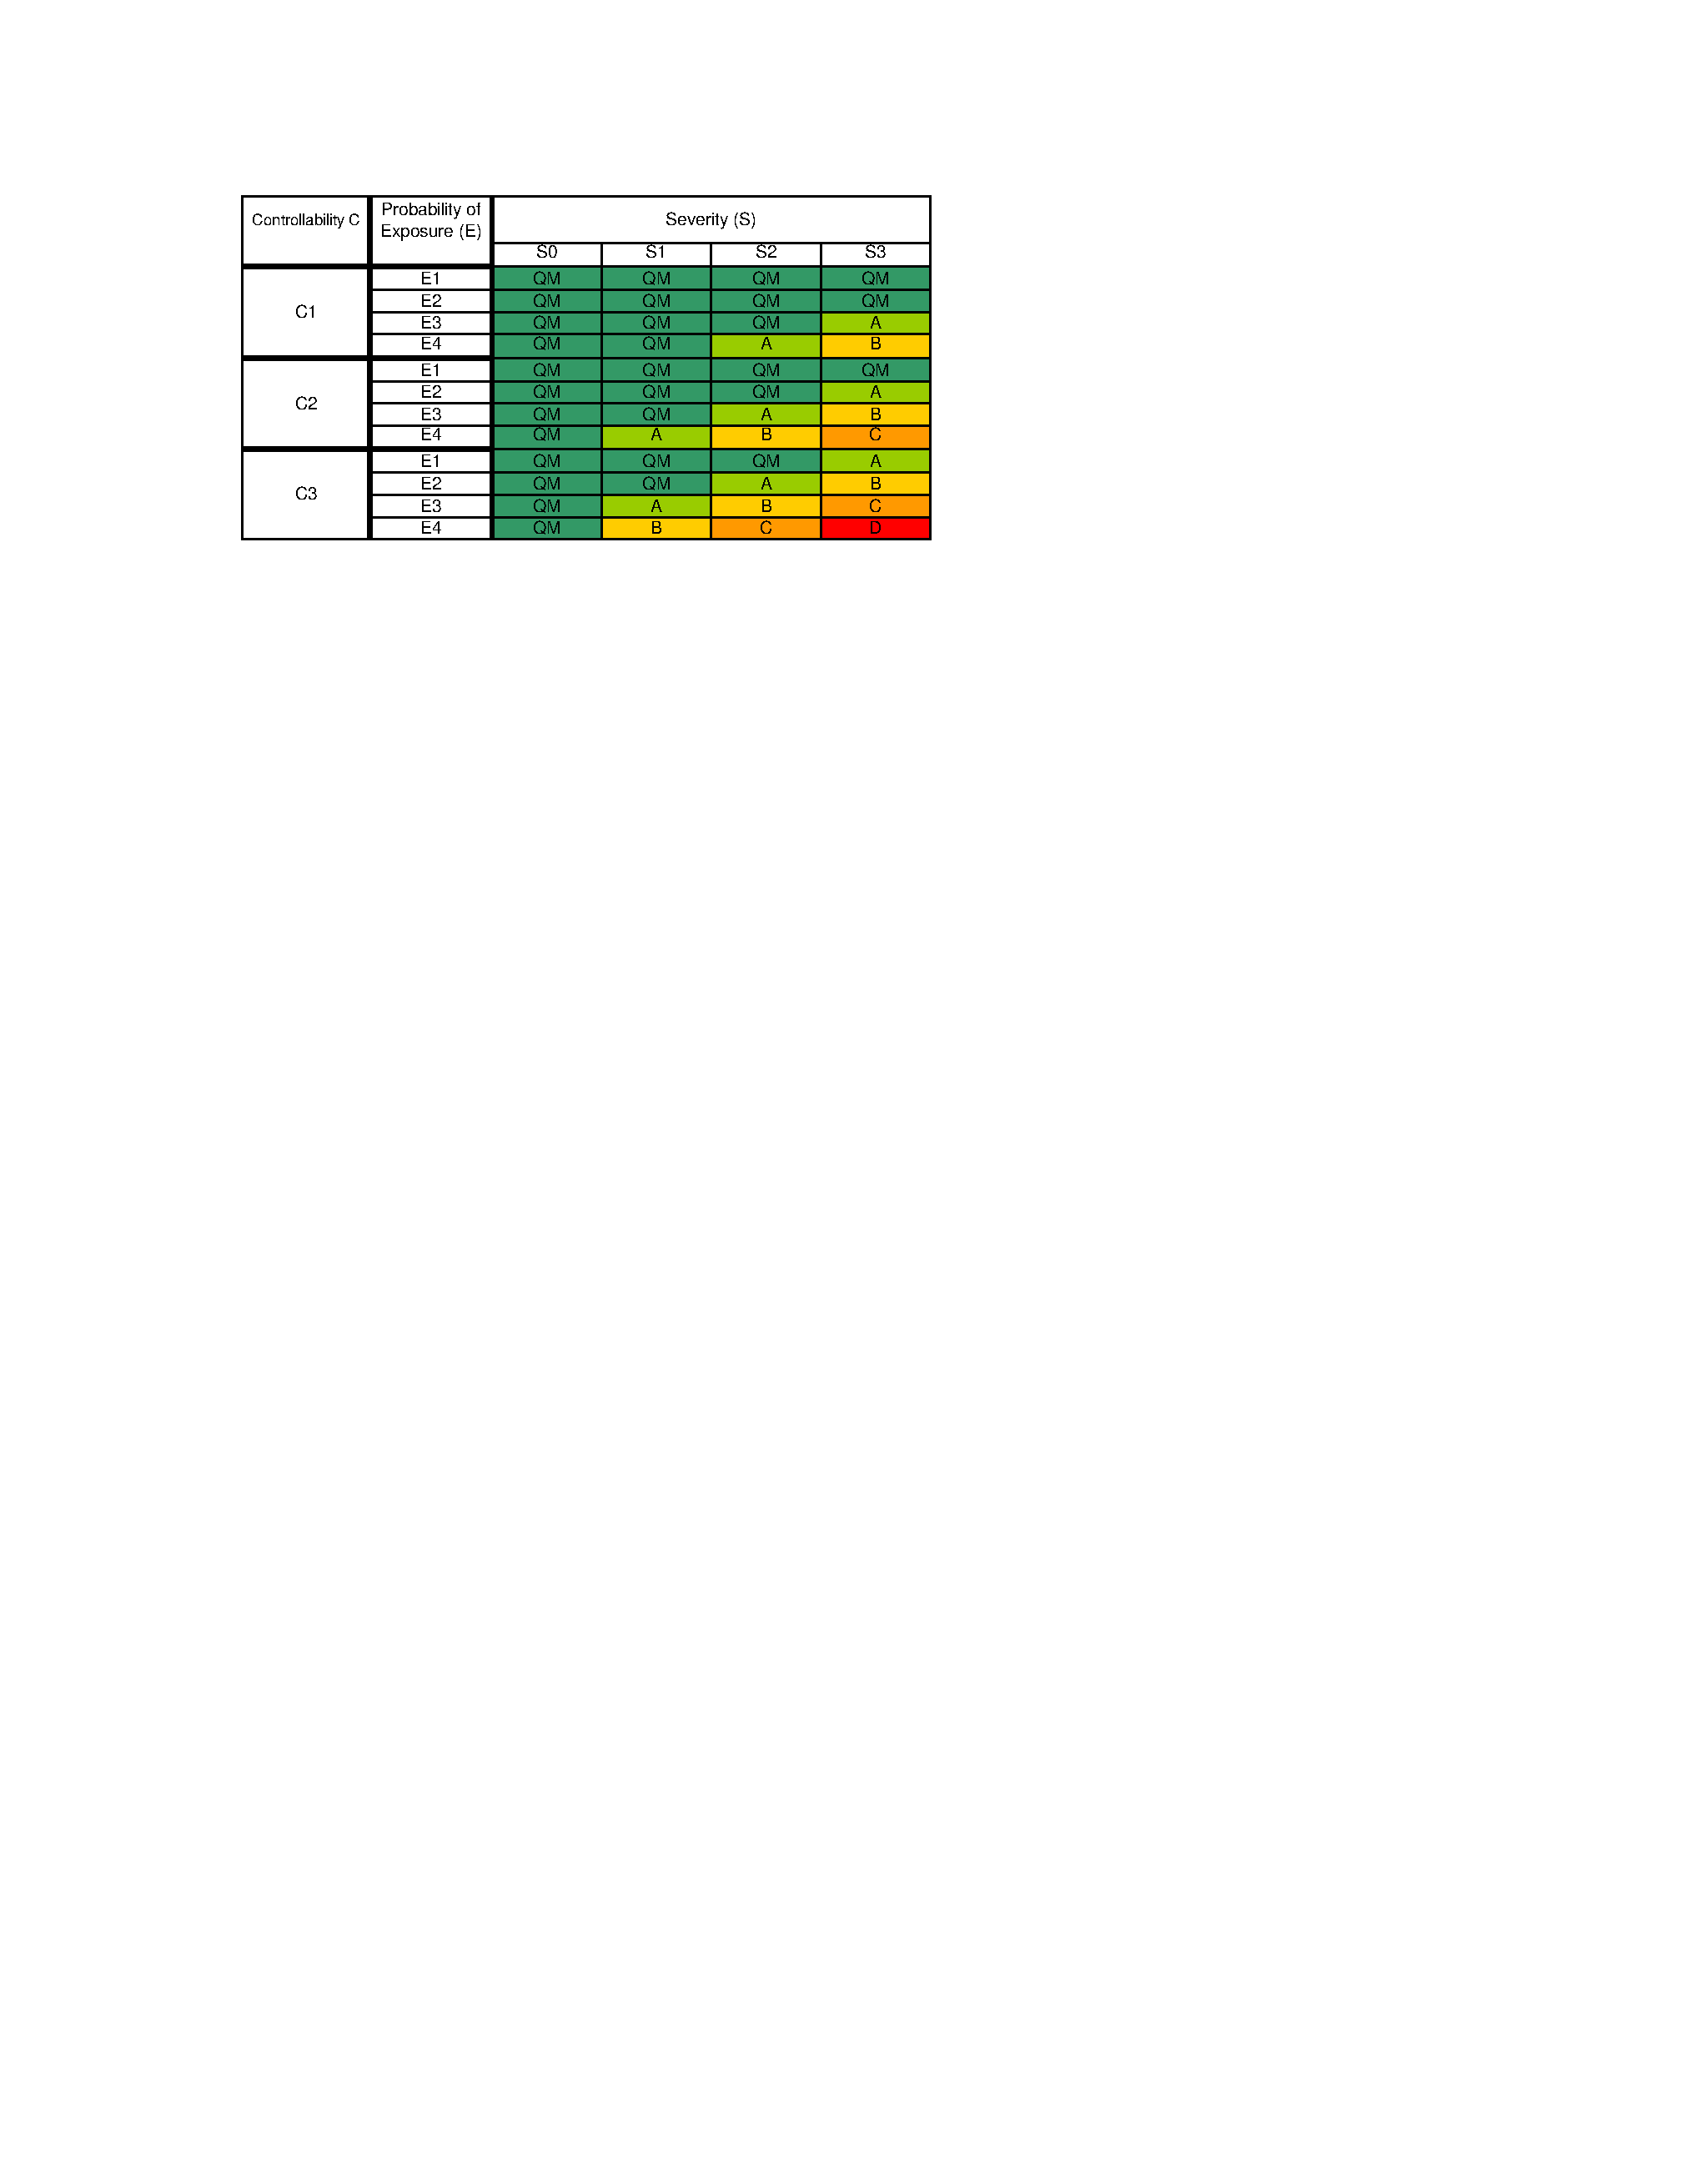
\includegraphics[width=0.9\linewidth]{./figures/ASIL}
	\caption{ASIL Risk Assessment Graph.}
	\label{Fig:ASILGraph}
\end{figure}

The ASIL methodology for risk assessment relies on the experts’ judgements of the three risk parameters. The ISO 26262 provides some general guidelines for assessing these parameters. However, the assessment is for the most part subjective and dependent on the experts who carry it out. Moreover, it is only capable of evaluating the risk of a single (hazardous) event within the context of a generic operational situation.

The objective of this paper is to introduce a method for analysis and quantification of the risk of a driving scenario taking into account the entire operational situations and their interrelation.

PAPER LAYOUT